
\import{./}{portada.tex}
\newpage
%so that the index can be shown
\tableofcontents
\printindex
\newpage
\begin{section}{Introduction}
	\begin{center}
		\begin{Large}
			before starting to install arch water linux make sure you have read this introduction page first
		\end{Large}
	\end{center}
	\begin{itemize}
		\item 
			if you already have installed arch linux into your computer, with a working boot you can skip into section 5
		\item
			the archiso installer has Arch Water operating system itself, with some 80\% of its functionalities, 
			also you are logged in as root, in the fututure it will have 100\% of if functionalities and you will be automaticly logged as root
		\item
			to open the terminal where will be typing all the commands you can press Control + Enter
		\item 
			to open a specific application you can just press <windows key> p and it will open a search bar
		\item
			once connected to the internet you can refer to the arch linux installation guide, because ArchWater linux in on top of arch linux you can follow this guide
			\url{https://wiki.archlinux.org/title/installation_guide#Install_essential_packages}
		\item 
			if you have a wired connection you can skip the "connecting to the internet" section
	\end{itemize}
\end{section}
\newpage
\begin{section}{Installation using the auto installer}
	this is suposed to be done using the auto installer that pops out
	\begin{itemize}
		\item
			you can move using the h,j,k,l for left,down,up,right
		\item
			since offline installation is the default first just quit out of the wifi by pressing the quit button
		\item
			pretty much everything is going to automatic, just enter the password for the root user and
			enter the username and the password for the username. accept all and start
	\end{itemize}
\end{section}
\begin{section}{connecting to the internet}
	\begin{Large}
		for connecting to the internet is very straight forward
		,just follow the following steps
	\end{Large}
	\begin{enumerate}
		\item 
			open the terminal as it says in (Control+Enter)
		\item
			start the network manager daemon
			\begin{minted}{sh}
				systemctl start NetworkManager
			\end{minted}
		\item
			enter the following command, which is a graphical user interface for wifi
			\begin{minted}{sh}
				nmtui
			\end{minted}
		\item 
			select Activate a connection
		\item 
			seelct your network and insert your password
		\item
			sync the time and date to avoid connection problems
			\begin{minted}{sh}
				timedatectl set-ntp true
			\end{minted}
		\item
			update the arch linux keyring (the installation medium is very old)
			\begin{minted}{sh}
				pacman -S archlinux-keyring
			\end{minted}

	\end{enumerate}
	note if pacman fails to download archlinux-keyring with 'core','extra','community' doesn't exist try installing the packages again with
	\begin{minted}{sh}
		pacman -Syy
	\end{minted}
	if the problem persist with 'could not open file' error try
	\begin{minted}{sh}
		rm -R /var/lib/pacman/sync/
		pacman -Syy
	\end{minted}
	to test the internet you can check the connection to google
	\begin{minted}{sh}
		ping www.google.com
	\end{minted}
\end{section}
\newpage
% ===================================== formatting the disks
\begin{section}{creating disk partitions and formatting them}
	this section is optional, if you don't know what you are doing, it si recommended to follow it.
	otherwise take any configuration you want, and use any tool that you like
	an example layout is shown below.
	in this sectio we will use the fdisk partitioning tool.
	here are some examples of valid layouts for arch linux
	\begin{Large}
		\begin{center}
			For UEFI method
		\end{center}
	\end{Large}
	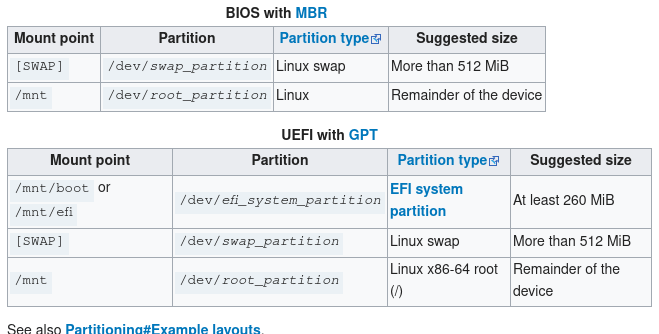
\includegraphics{partitionTablesExamples.png}
	\begin{minted}{sh}
		# for listing the partitions
		#room loop airoot may be ignored
		# you can see which drive is where you want to install it because of the size
		# most likely is gonna be /dev/sda
		fdisk -l
		# now select the drive, it may be different in your case
		fdisk /dev/sda
		# to see all the commands available you can just press m
		m
		# first delete all partitions
		# repeat the following tree commands as many times as necesary
		d
		<enter>
		<enter>
		# press g for creating a new gpt partition table
		g
		#### create the efi partition 
		# press n to create new partition
		n
		# press enter for default number identifire
		<enter>
		# press enter for default first sector
		<enter>
		# git 500 Mega bites to the partition
		+500M
		# press t to change the partition type
		t
		# press the number identifier of your partition in this case 1
		1
		# you can press L to see the list of all the partition types,
		# or just press 1 which is the efi partition type
		1
		### now create the swap partition
		# n for new partition
		n
		# enter for default number identifier
		<enter>
		# enter for default starting sector
		<enter>
		# give it 600 MB
		+600M
		# change the type
		t
		# press the number identifier of your partition in this case 2
		2
		# (optional) list all partition types available
		L
		# linux swap is number 19 so...
		19
		#### create the main partition
		# n for new partition
		n
		# leave all the defaults in this one
		<enter>
		<enter>
		<enter>
		# finally check that the partition table is correct comparing it to the images of GPT
		p
		# then write changes
		# warning all data will be lost when writing
		w
		## now format the partitions you just created
		# format the EFI partition
		mkfs.fat -F32 /dev/sda1
		# warning I am using sda3 but you should use your main partition
		mkfs.ext4 /dev/sda3
		# for the swap partition just mkswap
		mkswap /dev/sda2
		# now mount the partitions

		#first mount the root partition
		mount /dev/sda3 /mnt
		# turn on swap
		swapon /dev/sda2
		# create the /etc/fstab file
		# this file is used for automaticly mount partitions 
		genfstab -U -p /mnt >> /mnt/etc/fstab
		# check if everything is fine 
		cat /mnt/etc/fstab
	\end{minted}
	\begin{Large}
		for non UEFI method
	\end{Large}
	\begin{minted}{sh}
		# look for partitions
		fdisk -l
		# choose the partition where you want to install the operating system
		# note, sda here is an example, you should choose the one you want
		fdisk /dev/sda
		# first delete all partitions
		# repeat the following tree commands as many times as necesary
		d
		<enter>
		<enter>
		# create a dos partition table
		o
		# note, if you are asked to delete a signature just accept
		# create the swap partition
		n
		# make it primary partition
		p
		<enter>
		# give it 4GB mega bytes
		+4GB
		# change the partition type
		t
		# if you want to list the partition you can press L
		L
		# otherwise just press 82 for linux swap partition
		82
		# now create the main partition 
		n
		# make it primary
		p
		<enter>
		# give it the whole size
		<enter>
		## now format the partitions and turn on the swap partition
		mkfs.ext4 /dev/sda2
		mkswap /dev/sda1
		# turn on the swap partition
		swapon /dev/sda1
		# mount the partitions
		mount /dev/sda2 /mnt
		# this file is used for automaticly mount partitions 
		genfstab -U /mnt >> /mnt/etc/fstab
		# check if everything is fine
		cat /mnt/etc/fstab
	\end{minted}
\end{section}
\newpage
% ============================================= Install arch linux
\begin{section}{Install Arch Linux}
	 the following sections will be a lot less verbose and much simpler
	 \begin{minted}{sh}
		 # there will be a file in the installation medium called packages.txt 
		 #just open a terminal and execute this command it will show the file
		 # now execute this command
		 # this command will download and install arch linux with a
		 #bunch of additional packages for everything to work correctly
		 # when rebooting
		 pacstrap /mnt \$(cat packages.txt)
		 # change the root into the current instalation
		 arch-chroot /mnt
		 # enable sshd
		 systemctl enable sshd
		 # enable networkManager for rebooting
		 systemctl enable NetworkManager
		 # create the initial ramdisk for the kernel
		 mkinitcpio -p linux-lts
		 # syncronise the clock
		 hwclock --systohc
		 # uncomment the line from /etc/locale.gen file that corresponds to your locale
		 nvim /etc/locale.gen (uncomment en_US.UTF-8)
		 # generate the locate you just uncommented
		 locale-gen
		 # create a password for root
		 passwd
		 # create a user for yourself
		 useradd -m -g users -G wheel <username>
		 # create a password for the user you just created
		 passwd <username>
		 # allow uses in the wheel group
		 EDITOR=nvim visudo
		 # in tha file uncomment \%wheel ALL=(ALL) ALL
	 \end{minted}
\end{section}
\newpage
% ============================================== Installing grub
\begin{section}{installing grub}
	finally all has been done, 
	but it still mising a boot manager
	\begin{Large}
		UEFI method
	\end{Large}
	\begin{minted}{sh}
		#rceate directory
		mkdir /boot/EFI
		#mount the efi partition
		mount /dev/sda1 /boot/EFI
		#install grub
		 grub-install --target=x86_64-efi --bootloader-id=grub_uefi --recheck
		 #create the locale directory for grub
		 mkdir /boot/grub/locale
		 #copy the locale file to locale directory
		 cp /usr/share/locale/en\@quot/LC_MESSAGES/grub.mo /boot/grub/locale/en.mo
		 #generate grub config file
		 cp /usr/share/locale/en\@quot/LC_MESSAGES/grub.mo /boot/grub/locale/en.mo
	\end{minted}
	% === non uefi

	\begin{Large}
		non UEFI method
	\end{Large}
	\begin{minted}{sh}
		# install grub
		grub-install --target=i386-pc --recheck /dev/sda
		# create the directory 
		mkdir /boot/grub/locale

		# copy the locale file to locale directory
		cp /usr/share/locale/en\@quot/LC_MESSAGES/grub.mo /boot/grub/locale/en.mo
		# generate grubs config file
		grub-mkconfig -o /boot/grub/grub.cfg

	\end{minted}

\end{section}
% Installing arch water linux
\newpage
\begin{section}{Installing ArchWater Linux}
now arch linux is fully working, is time to install arch water linux
\begin{minted}{sh}
	# select the folder of your user
	cd home/<username>
	#git clone the repository 
	git clone https://github.com/Virgilio-AI/ArchWater-AutoInstaller.git archAutoInstaller
	# exit arch-chroot
	exit
	# reboot and you sould be logged into arch linux
	reboot
	# now log in with your user and password
	#
	# maybe you will need to connect to the internet again
	##
	#

	cd archAutoInstaller
	sudo sh ArchWater-AutoInstaller.sh
	# follow the installer and you should be good to go
\end{minted}
\end{section}

